\documentclass[aspectratio=169]{beamer}

\usepackage[T1]{fontenc}
\usepackage[utf8]{inputenc}
\usepackage{lmodern}
\usepackage{amsmath,amssymb}
\usepackage{booktabs}
\usepackage{tikz}
\usetikzlibrary{positioning, arrows.meta}

\usetheme{Madrid}
\usecolortheme{seahorse}
\setbeamertemplate{navigation symbols}{}
\setbeamertemplate{footline}[frame number]

\title{StoCFL}
\subtitle{Stochastic Clustered Federated Learning: clusterização estocástica com participação parcial}
\author{luiz2801}
\institute{Repositório \texttt{cfl\_stocfl}}
\date{Baseado em Zeng et al. (2025)}

\begin{document}

\begin{frame}
  \titlepage
\end{frame}

\begin{frame}{Roteiro}
  \begin{enumerate}
    \item Problema: clusterização com participação parcial
    \item Representação do cliente: o gradiente normalizado $\Psi$
    \item Clusterização estocástica (SFCC): fusão de clusters pelo cosseno
    \item Treino bi-nível (Bi-CFL): modelo de cluster e modelo global
    \item Casos limite, cenários do repositório e resultados
    \item Correções feitas, limitações e comparação com o CFL
  \end{enumerate}
\end{frame}

\section{Problema}

\begin{frame}{Por que o StoCFL}
  \begin{itemize}
    \item Em FL real, só uma fração dos clientes participa de cada rodada.
    \item O CFL clássico precisa de todos os clientes ao mesmo tempo, para medir as atualizações
      de cada cluster.
    \item Métodos anteriores exigiam o número de clusters $K$ como conhecimento prévio.
    \item Com pouca amostragem, um cluster pequeno gera um modelo ruim, porque não troca
      informação com os outros.
  \end{itemize}
\end{frame}

\begin{frame}{Suposição e objetivo}
  \begin{itemize}
    \item Existem $N$ clientes, cada um com dados $D_i$, e $K$ distribuições latentes $P_k$.
    \item O servidor \textbf{não conhece} $K$.
    \item Objetivo: clusterizar os clientes com amostragem parcial, e treinar um modelo por cluster
      que se beneficie dos outros clusters.
  \end{itemize}
\end{frame}

\section{Representação do cliente}

\begin{frame}{O extrator $\Psi$}
  \[
    \Psi(D) = \frac{\nabla_{\psi}\,\ell(\psi; D)}{\left\|\nabla_{\psi}\,\ell(\psi; D)\right\|}
  \]
  \begin{itemize}
    \item $\psi$ é a \textbf{âncora}: o modelo inicial $\omega_0$, que \textbf{nunca muda}.
    \item O gradiente é calculado no dataset inteiro do cliente, \textbf{sem treinar}.
    \item Cada cliente é observado \textbf{uma única vez}, na primeira vez em que é sorteado.
  \end{itemize}
\end{frame}

\begin{frame}{Por que dá para comparar clientes de rodadas diferentes}
  \begin{itemize}
    \item A âncora e a função de perda são fixas e iguais para todos.
    \item Então $\Psi(D_i)$ é a mesma função de $D_i$, em qualquer rodada.
    \item A similaridade é o cosseno:
      \[
        \cos\big(\Psi(D_i), \Psi(D_j)\big) = \frac{\Psi(D_i)\cdot\Psi(D_j)}{\|\Psi(D_i)\|\,\|\Psi(D_j)\|}
      \]
    \item Clientes com a mesma distribuição produzem $\Psi$ quase paralelos.
  \end{itemize}
\end{frame}

\section{Clusterização estocástica}

\begin{frame}{Uma rodada do SFCC}
  \begin{enumerate}
    \item O servidor sorteia $m$ clientes e agrupa-os pelo cluster atual.
    \item Para cada cluster sorteado, o centro é a \textbf{média dos $\Psi$ de todos os membros},
      não só dos sorteados na rodada.
    \item Calcula-se o cosseno entre os centros de todos os pares de clusters sorteados.
    \item Os pares são percorridos do maior cosseno ao menor. Se $\cos > \tau$, os dois clusters
      são \textbf{fundidos}. No primeiro par que não passa de $\tau$, a rodada para.
  \end{enumerate}
\end{frame}

\begin{frame}{Fusão em cadeia (single linkage)}
  \begin{center}
    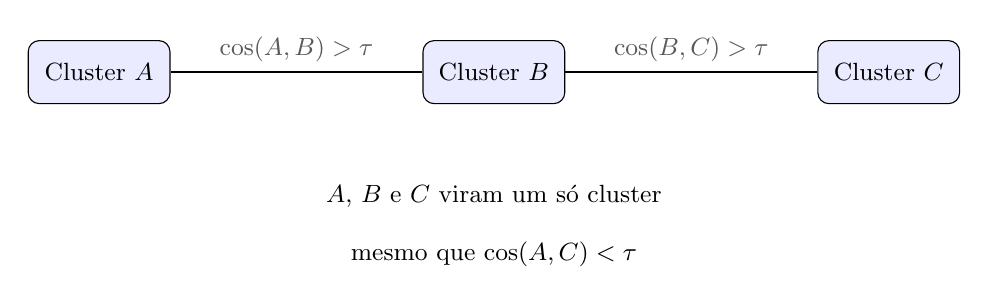
\begin{tikzpicture}[
      cl/.style={draw, rounded corners, fill=blue!8, font=\small, minimum width=1.8cm, minimum height=0.8cm},
      lk/.style={font=\small, midway, above, text=gray!70!black},
      edge/.style={thick, -{Stealth}}]
      \node[cl] (A) {Cluster $A$};
      \node[cl, right=3.2cm of A] (B) {Cluster $B$};
      \node[cl, right=3.2cm of B] (C) {Cluster $C$};
      \draw[thick] (A) -- node[lk] {$\cos(A,B) > \tau$} (B);
      \draw[thick] (B) -- node[lk] {$\cos(B,C) > \tau$} (C);
      \node[font=\small, below=0.9cm of B] (res) {$A$, $B$ e $C$ viram um só cluster};
      \node[font=\small, below=0.2cm of res] (note) {mesmo que $\cos(A,C) < \tau$};
    \end{tikzpicture}
  \end{center}
  \vspace{0.2em}
  \begin{itemize}
    \item A fusão é transitiva, então o resultado é \emph{single linkage} com corte em $\tau$.
    \item Fusões são \textbf{irreversíveis}: o código nunca divide um cluster.
  \end{itemize}
\end{frame}

\begin{frame}{Com o tempo, o número de clusters converge}
  \begin{itemize}
    \item Clientes com a mesma distribuição vão se juntando, rodada após rodada.
    \item O número de clusters tende ao número real $K$ de distribuições, se $\tau$ estiver bem escolhido.
    \item No artigo, a avaliação é qualitativa: t-SNE de $\Psi$ e a curva do número de clusters.
      Não há ARI, NMI ou pureza.
  \end{itemize}
\end{frame}

\section{Treino bi-nível}

\begin{frame}{Bi-CFL: dois modelos por cliente}
  Para cada cliente sorteado, com $\omega$ o modelo global:
  \begin{itemize}
    \item \textbf{Modelo do cluster $\theta_k$:} perda de classificação mais termo proximal
      \[
        f_k(\theta_k) + \frac{\lambda}{2}\,\|\theta_k - \omega\|^2
      \]
    \item \textbf{Modelo global $\omega$:} SGD puro, a partir do mesmo $\omega_t$ da rodada, com FedAvg.
  \end{itemize}
  \vspace{0.4em}
  Ao fim da rodada, o servidor faz a média dos modelos globais e dos modelos de cada cluster.
\end{frame}

\begin{frame}{Casos limite}
  \begin{center}
    \begin{tabular}{@{}ll@{}}
      \toprule
      Configuração & Equivale a \\
      \midrule
      $\lambda = 0$ & CFL convencional, com clusters independentes \\
      $\lambda$ grande & Modelos de cluster próximos do modelo global \\
      $\tau = 1$ & Nenhuma fusão: um cluster por cliente, como o Ditto \\
      $\tau = -1$ & Um único cluster, como o FedProx \\
      $\lambda = 0$ e $\tau = -1$ & FedAvg \\
      \bottomrule
    \end{tabular}
  \end{center}
\end{frame}

\section{Algoritmo do servidor}

\begin{frame}{Uma rodada, do ponto de vista do servidor}
  \begin{enumerate}
    \item Sorteia \texttt{num\_per\_round} clientes.
    \item Para cada sorteado sem $\Psi$: calcula e guarda o gradiente normalizado na âncora.
    \item Recalcula os centros dos clusters sorteados e funde os pares com cosseno maior que $\tau$.
    \item Se \texttt{train = 1}: treina o modelo de cluster e o global de cada sorteado.
    \item Agrega com FedAvg e registra as acurácias.
  \end{enumerate}
\end{frame}

\section{Repositório e resultados}

\begin{frame}{Cenários do repositório}
  \begin{tabular}{@{}lll@{}}
    \toprule
    Script & Cenário & Procedimento \\
    \midrule
    \texttt{StoCFL-FCC.py} & Rotated, shifted, label skew, feature skew & só FCC (\texttt{--train 0}) \\
    \texttt{StoCFL-FCC+CFL.py} & Rotated MNIST e CIFAR-10 & FCC + Bi-CFL \\
    \texttt{StoCFL-FEMNIST.py} & FEMNIST (LEAF) & FCC + Bi-CFL \\
    \bottomrule
  \end{tabular}
  \vspace{0.8em}

  Valores do artigo para o cenário Rotated: $\tau = 0{,}5$, $\lambda = 0{,}05$, 5 sementes.
\end{frame}

\begin{frame}{Resultados publicados}
  \begin{itemize}
    \item Rotated MNIST e CIFAR-10, Shifted MNIST, FEMNIST e FedCelebA, com comparação com FedAvg,
      FedProx, Ditto, IFCA, CFL e FedSEM.
    \item Ablação de $\lambda$ e de $\tau$.
    \item Clientes novos, com 30\% dos clientes de fora do treino.
  \end{itemize}
  \vspace{0.6em}
  \begin{alertblock}{Atenção}
    Nenhum baseline está implementado no repositório. As tabelas do artigo não podem ser
    reproduzidas só com este código.
  \end{alertblock}
\end{frame}

\section{Correções e limitações}

\begin{frame}{Correções feitas no repositório}
  O código foi ajustado para seguir o texto do artigo:
  \begin{itemize}
    \item $\Psi$ passou a ser o gradiente normalizado na âncora, e não a diferença de pesos.
    \item O centro do cluster usa todos os membros, como na Eq. 2.
    \item O modelo global é o FedAvg de clientes que partem do mesmo $\omega_t$.
      Antes, cada cliente partia do resultado do anterior.
    \item Limiar de fusão estrito, $\cos > \tau$. Modelos de cluster começam em $\omega_0$.
  \end{itemize}
  \vspace{0.4em}
  \alert{Com isso, os resultados ficam abaixo das tabelas publicadas.} Há indícios de que as
  tabelas vieram do código original, mas isso é uma inferência, não uma prova.
\end{frame}

\begin{frame}{Limitações conhecidas}
  \begin{itemize}
    \item Fusões são irreversíveis, e não há divisão de clusters.
    \item Cada cliente sorteado treina duas vezes por rodada: no cluster e no global.
    \item Inferência para clientes novos não está implementada.
    \item Não há análise teórica: só evidência empírica.
    \item No \texttt{StoCFL-FCC.py}, o caminho \texttt{--train 1} não funciona para todos os cenários.
  \end{itemize}
  \vspace{0.4em}
  \small Lista completa: \texttt{docs/guia.md}, seção 4.12.
\end{frame}

\begin{frame}{StoCFL e CFL, lado a lado}
  \begin{center}
    \begin{tabular}{@{}lll@{}}
      \toprule
      Aspecto & CFL & StoCFL \\
      \midrule
      Direção & divisivo & aglomerativo \\
      Participação & todos os clientes & parcial \\
      Sinal de similaridade & $\Delta W$ da rodada & $\Psi$, calculado uma vez \\
      Quando agrupa & após o FL convergir & desde a primeira rodada \\
      Controle do número de clusters & $\varepsilon_1$, $\varepsilon_2$ & $\tau$ \\
      Garantia teórica & Teorema da Separação & só empírica \\
      \bottomrule
    \end{tabular}
  \end{center}
\end{frame}

\begin{frame}{Referência}
  \begin{itemize}
    \item D. Zeng, X. Hu, S. Liu, Y. Yu, Q. Wang e Z. Xu. \emph{StoCFL: A stochastically
      clustered federated learning framework for Non-IID data with dynamic client participation.}
      Neural Networks, 187, 2025, 107278. arXiv:2303.00897.
  \end{itemize}
\end{frame}

\end{document}
